\fancyhf{}
\setlength{\headheight}{14.49998pt}
\lhead{\textsl{\footnotesize{\nouppercase{\rightmark}}}}
\rhead{\textsl{\footnotesize{\nouppercase{\leftmark}}}}

\cfoot{\thepage}
\rfoot{\textsl{\footnotesize}}

\chapter{AI and System Design}

\section{Introduction}
This chapter presents the core design concepts that translate the requirement baseline into a coherent technical solution. It explains how the chatbot is structured as a coordinated architecture linking user channels, backend orchestration, AI inference, and persistence mechanisms. Particular attention is given to interoperability across Meta messaging channels through webhook-driven communication, and to the design logic that keeps responses coherent, safe, and commercially useful.

Beyond structural description, the chapter justifies key AI and system design decisions, including model integration strategy, prompt-based behavioral control\cite{liu2023prompting_survey}, tool-assisted response generation, and conversation-state management backed by database persistence. This perspective is important because it clarifies the trade-offs that balance responsiveness, reliability, security, and maintainability.

\section{System Architecture Design}
The global architecture follows a layered, event-driven design centered on a Node.js\cite{nodejs_docs} Express\cite{express_docs} orchestration core. At the edge, user interactions originate from Messenger, Instagram, and WhatsApp, then arrive as webhook events that trigger a unified processing flow\cite{meta_webhooks_docs}. The orchestration layer coordinates pre-processing, context retrieval, AI invocation, and response dispatch so that all channels share one consistent decision core while preserving channel-specific payload formatting.

A key concept in this architecture is separation of concerns. Channel integration is handled by dedicated adapters, AI reasoning is handled by model and tool orchestration, and state continuity is handled by a persistence layer. The database design therefore plays a central role by storing conversation context, handoff cooldown status, and operational metadata required for coherent multi-turn behavior.

\begin{figure}[H]
    \centering
    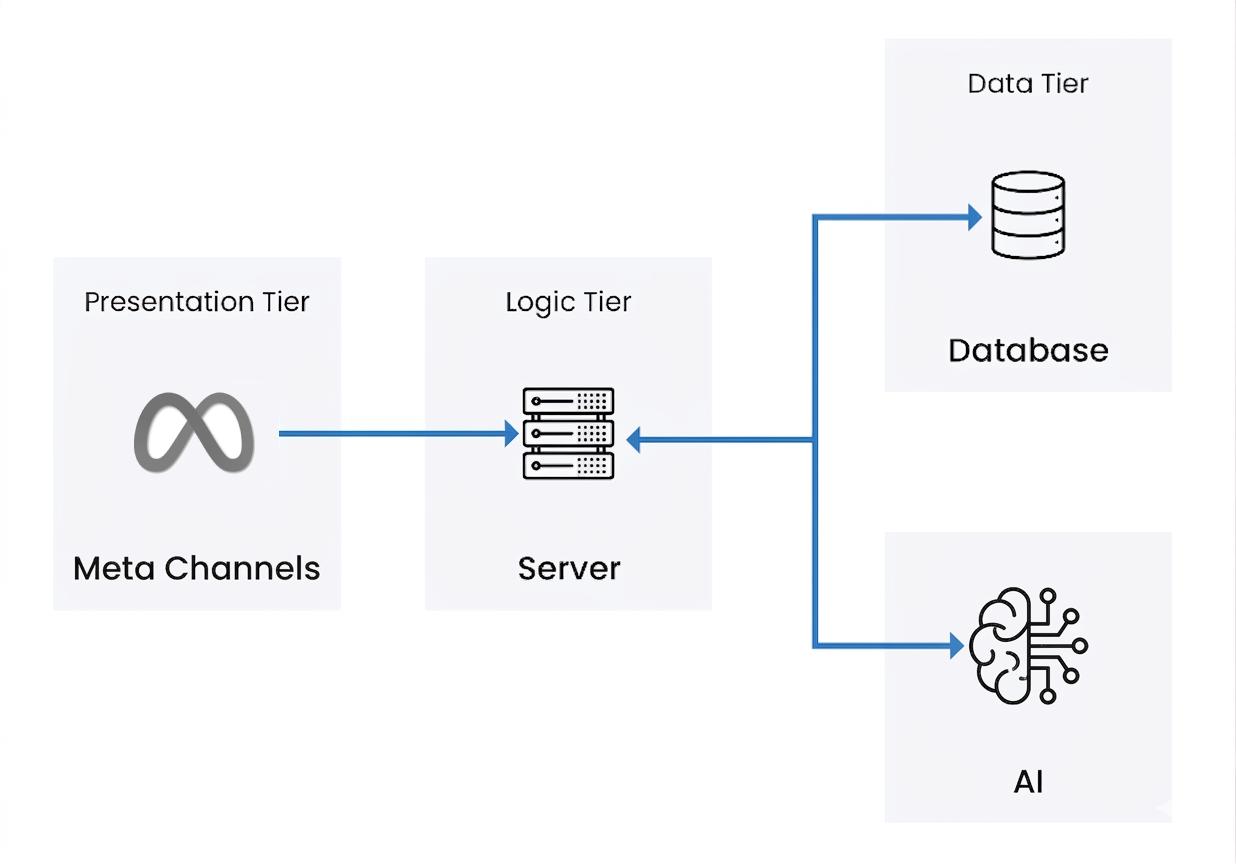
\includegraphics[width=0.95\textwidth]{Images/architecture.png}
    \caption{System Architecture view showing Meta channel integration, backend orchestration, AI interaction, and the persistence layer.}
    \label{fig:architecture}
\end{figure}

\section{Channel Integration Design}
Channel integration design follows a unified strategy that treats Messenger, Instagram, and WhatsApp as distinct transport channels connected to the same conversational core. Although each platform has specific payload structures and configuration requirements\cite{meta_messenger_platform_docs}\cite{meta_instagram_messaging_docs}\cite{meta_whatsapp_cloud_api_docs}, inbound events are normalized into a common internal message model before AI processing. This concept avoids duplicated business logic and keeps response behavior consistent regardless of entry channel.

At integration level, webhook endpoints act as event ingress points and enforce platform verification, message authenticity checks, and channel routing\cite{meta_webhooks_docs}. Once validated, messages follow the same orchestration path: acknowledgment signals are emitted, context is recovered, AI generation is executed, and the final response is transformed back into the channel-specific outbound format. By isolating channel adapters from core reasoning logic, the system can support channel-specific evolution without destabilizing global assistant behavior.

\begin{figure}[H]
    \centering
    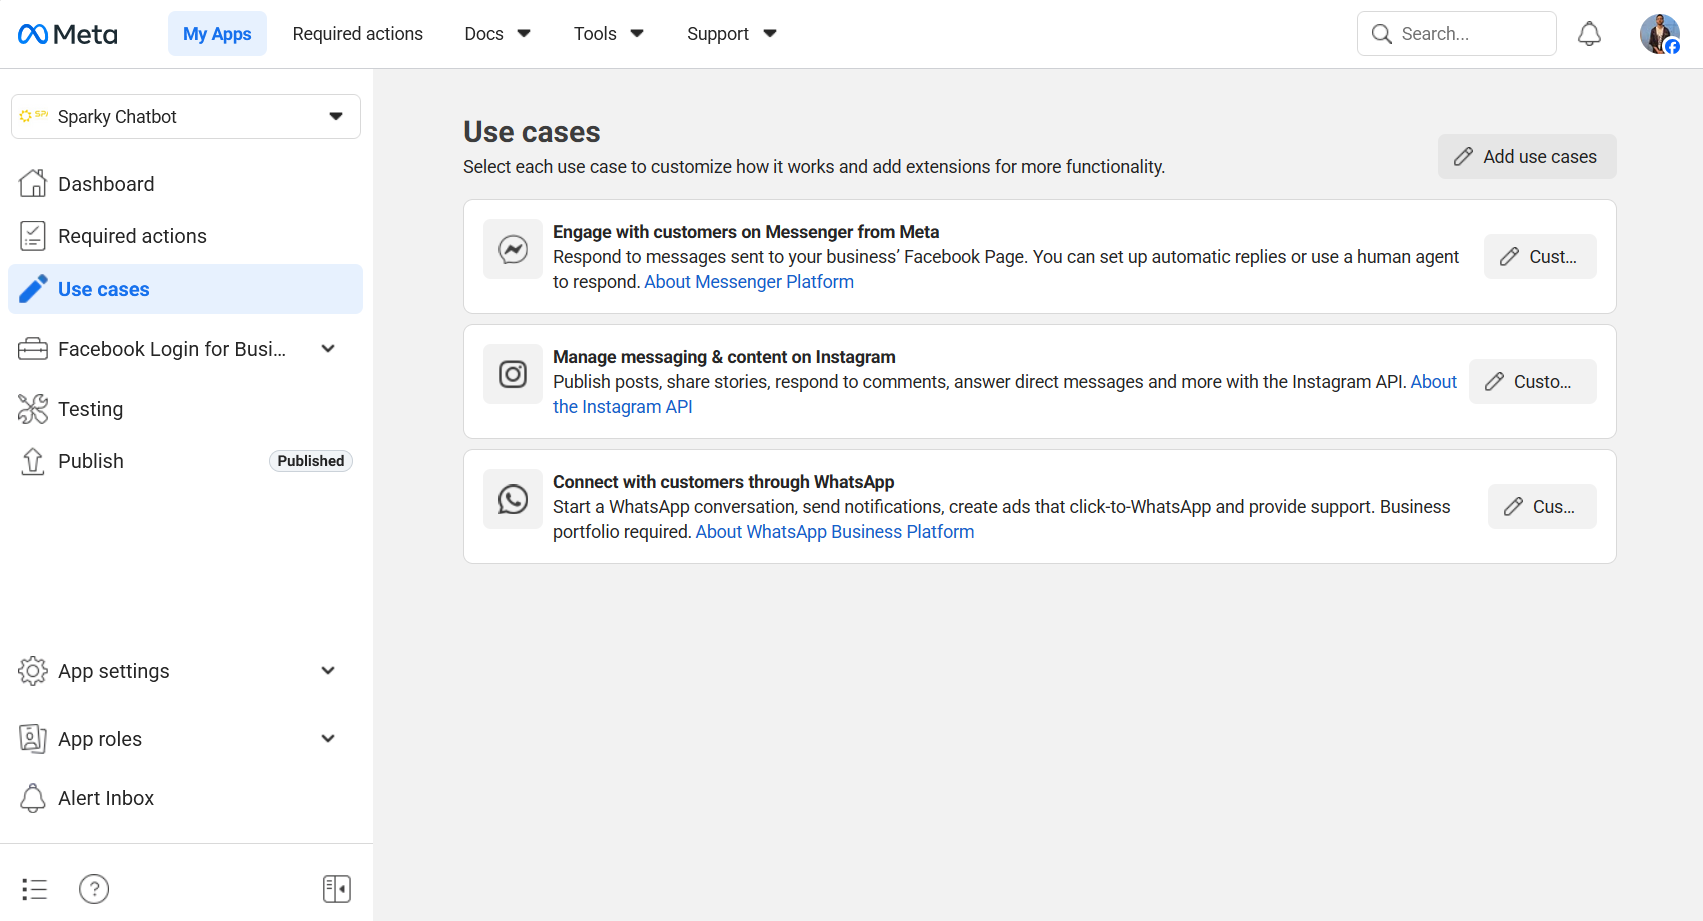
\includegraphics[width=0.95\textwidth]{Images/meta_dashboard.png}
    \caption{Meta developer dashboard showing Messenger, Instagram, and WhatsApp "use cases".}
    \label{fig:meta-dashboard}
\end{figure}

\section{Backend Design}
The backend design is based on an Express orchestration layer responsible for transforming incoming channel events into controlled conversational actions. Its structure follows modular design concepts: webhook handlers manage channel entry points, processing services execute conversation logic, and outbound adapters build platform-compliant response payloads. This separation reduces coupling between transport-specific code and core assistant behavior, which supports maintainability and future extension.

At runtime, the backend follows a deterministic processing design: message reception, validation, context loading, AI request orchestration, response formatting, and state persistence. The database is used as the authoritative source for user context and conversation continuity, including cooldown tracking after human-handoff requests. Cross-cutting concerns such as security filtering and fallback behavior are applied as policy gates inside this pipeline, resulting in a predictable flow across channels under variable user input and platform-side event patterns.

\section{AI Interaction Design}
AI interaction design defines how language reasoning, business constraints, and conversation continuity are combined into a single response-generation concept. Instead of treating the model as an isolated component, the design positions it inside a controlled pipeline where prompt rules, tool access, and persisted context jointly shape output quality.

\subsection{Model Selection and Integration}
Model selection is guided by a balance between linguistic quality, instruction-following consistency, latency constraints, and integration feasibility. The adopted design relies on a modern Transformer-based large language model family\cite{vaswani2017attention} accessed through a service-oriented API layer, which allows response generation to remain decoupled from channel transport and backend routing concerns.

Integration design emphasizes a clear boundary between orchestration logic and model invocation logic. The backend prepares normalized inputs (message content, channel metadata, and conversation context), submits them to the AI layer, then processes the model output under policy constraints before channel delivery. This concept supports maintainability because model-related adjustments can be made with minimal impact on surrounding architecture.

\subsection{Prompt Engineering Strategy}
Prompt engineering is treated as a design control mechanism rather than a simple text instruction. The system prompt is structured to encode role definition, behavioral boundaries, commercial guidance objectives, and refusal rules for unsafe requests\cite{liu2023prompting_survey}. This design choice is especially relevant in the current project context, where domain data is not sufficient for robust fine-tuning.

Prompting also enforces output consistency across channels by keeping one shared instruction baseline regardless of message origin. Within this baseline, the assistant is configured to respond primarily in French or Tunisian dialect, selected according to the user's language and conversational context. As a result, differences between Messenger, Instagram, and WhatsApp remain transport-level concerns, while assistant behavior remains conceptually uniform at reasoning level.

\subsection{Tool-Calling Strategy}
Tool-calling design addresses the gap between fluent language generation and domain-grounded commercial precision. Instead of relying exclusively on free-form generation, the AI layer can request structured tool outputs when a response depends on company-specific rules or quote-related calculations. This concept reduces unsupported claims and improves answer reliability in business-critical interactions.

At system level, tool calls are orchestrated as controlled steps inside the same AI request cycle: detect need, retrieve structured result, then compose final response. This design keeps reasoning and data access aligned while preserving a single conversational experience for the user.

\begin{figure}[H]
    \centering
    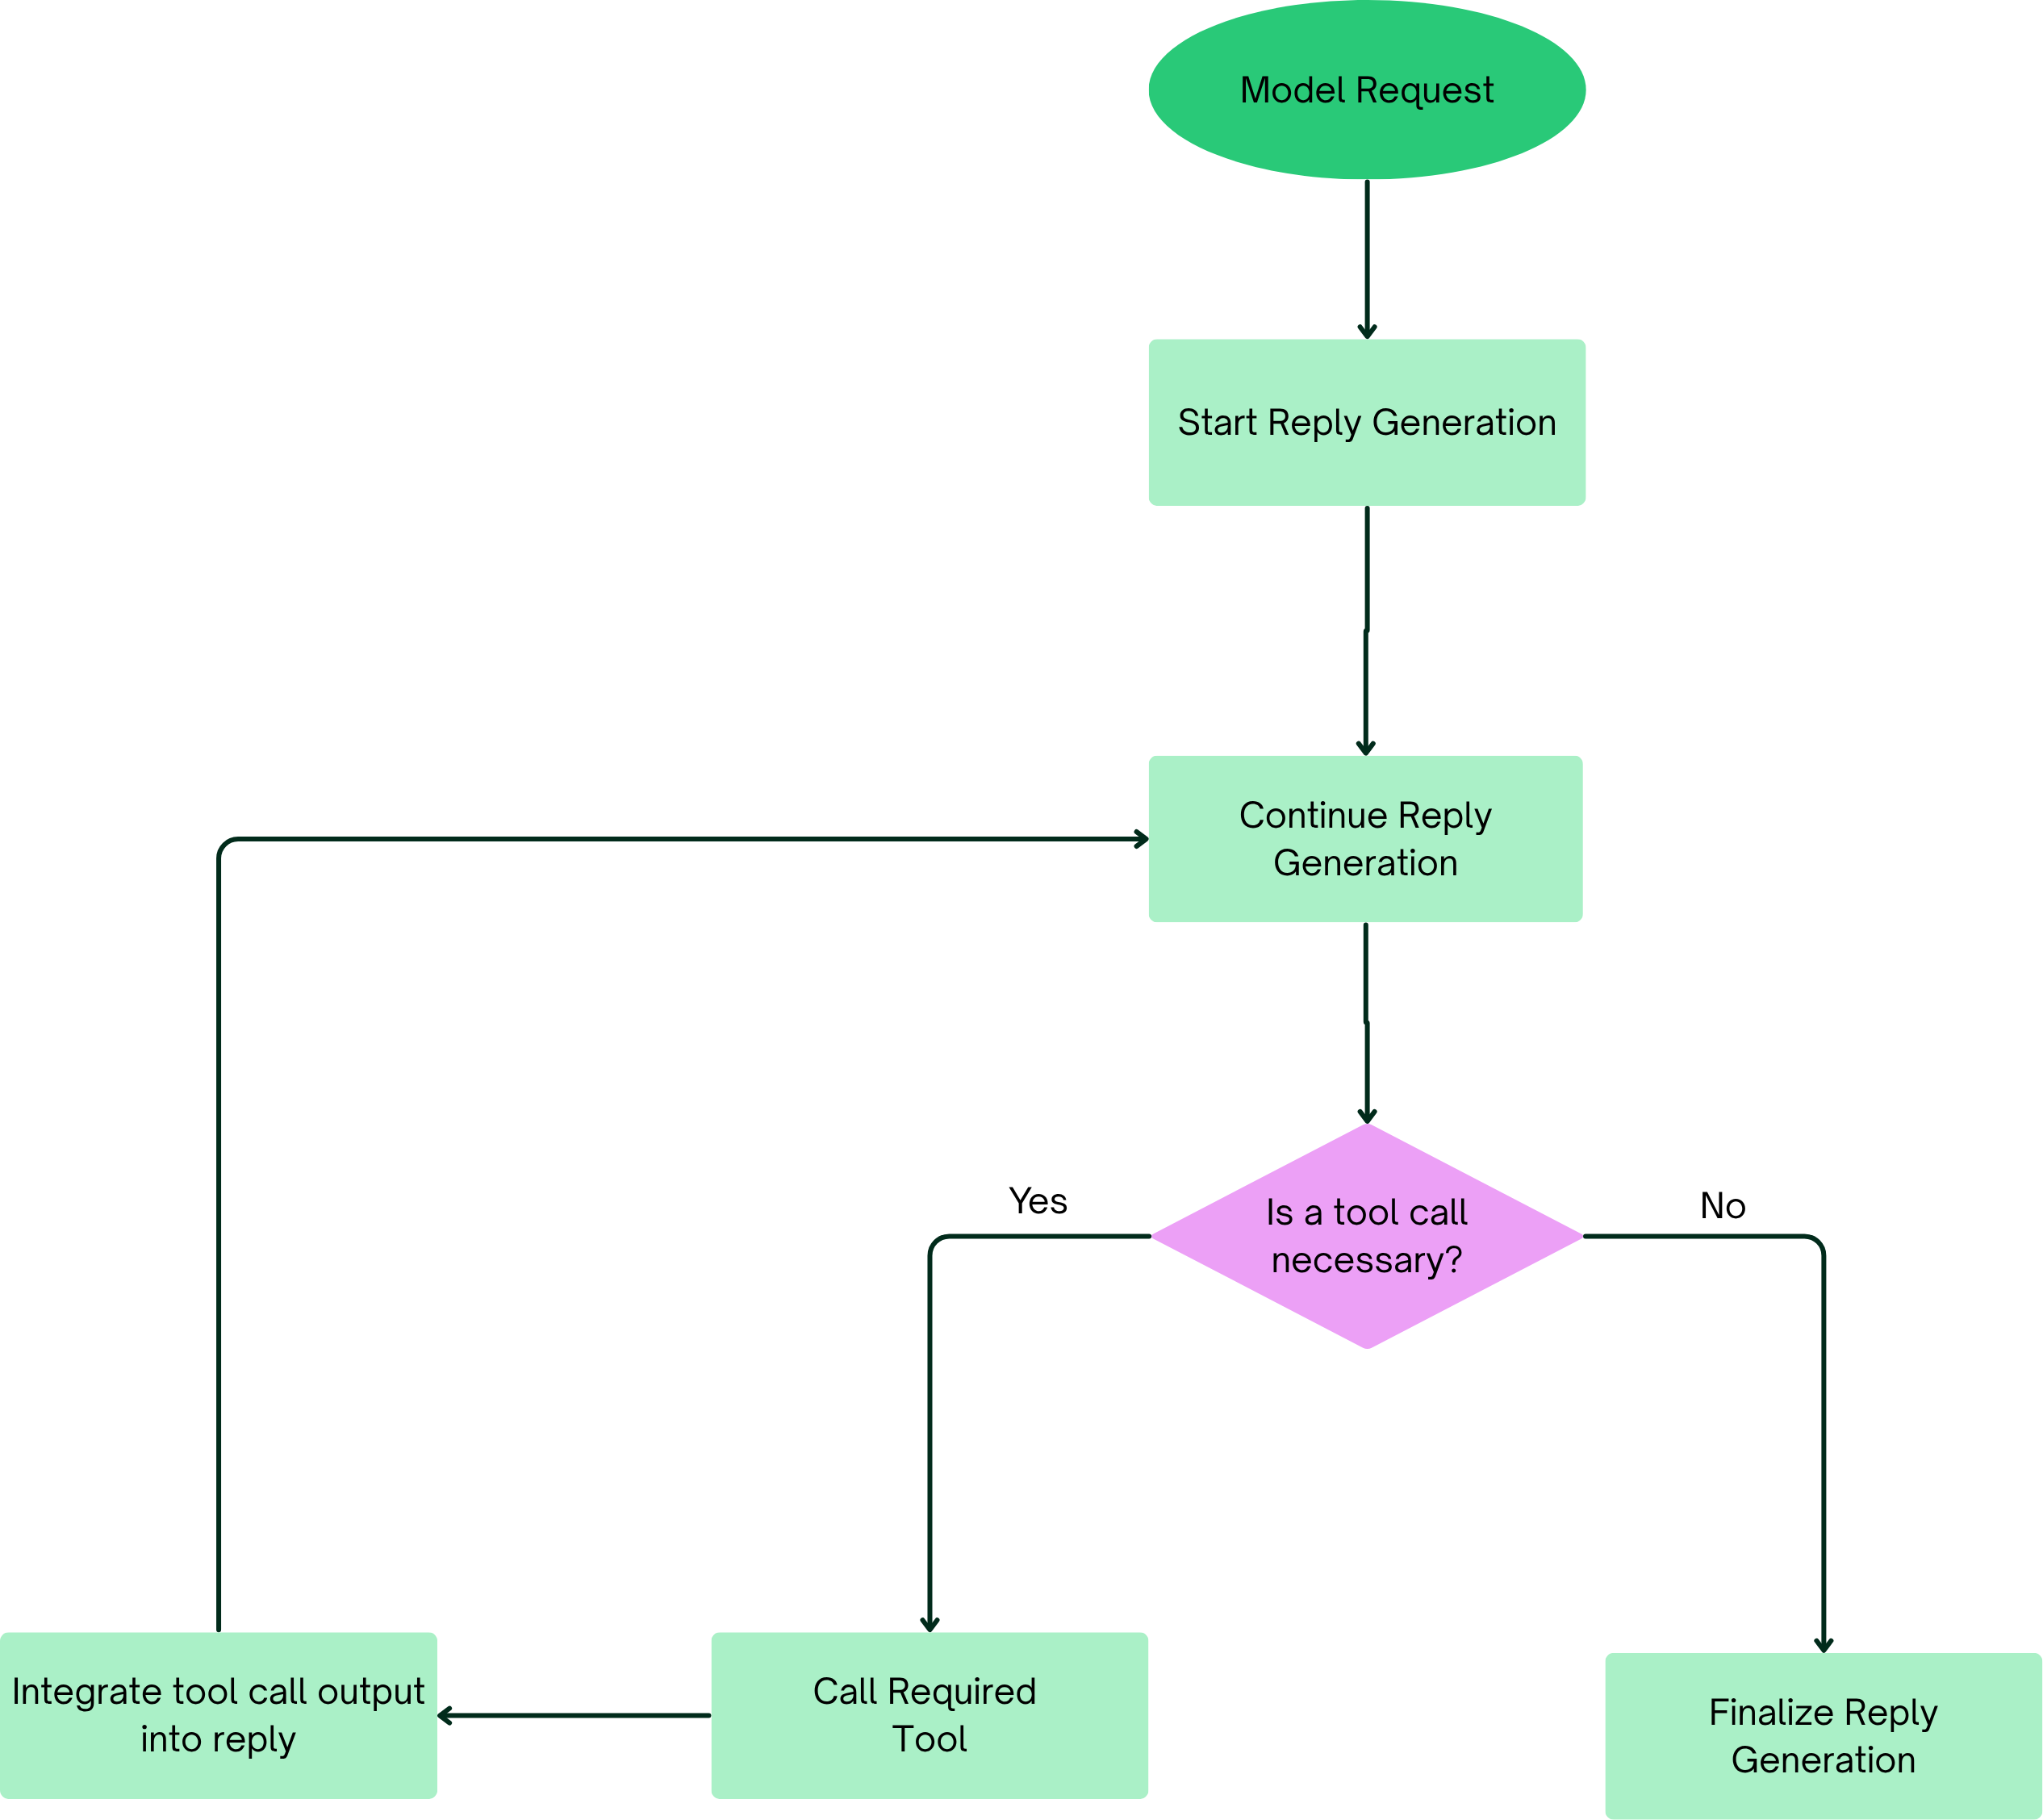
\includegraphics[width=0.8\textwidth]{Images/tool_call_simplified.png}
    \caption{Simplified tool-calling flow within AI response generation.}
    \label{fig:tool-call-simplified}
\end{figure}

\subsection{Conversation Context and Memory Handling}
Conversation context design is based on continuity across multi-turn exchanges. A key concept is that LLMs are stateless at inference time\cite{srinivasan2026stateless_decision_memory}: they do not keep an internal long-term memory of previous turns, and each output is generated only from the input currently provided to the model. For this reason, the design feeds the relevant conversation history again at every response cycle, together with the latest user message, so that reasoning remains coherent across the full dialogue.

The database plays a central design role in this layer by storing user-specific conversation history, channel identifiers, and operational state flags such as human-handoff cooldown status. AI interaction therefore depends on database-backed context retrieval before generation and database-backed state updates after generation, ensuring that each new response remains aligned with prior interaction state.

\section{Operational Design}
Operational design defines how the system preserves safe behavior and service continuity under real-world usage conditions. The objective is not only to produce correct responses in nominal cases, but also to maintain controlled behavior when inputs are adversarial, ambiguous, incomplete, or affected by platform-side instability.

\subsection{Security and Safety Mechanisms}
Security and safety are driven by layered control concepts applied before and after AI generation. At input level, the design screens messages for instruction-overriding patterns and blocks requests that attempt to expose confidential internal guidance. At output level, responses are constrained by policy-aligned prompt rules and business boundaries so that generated content remains commercially relevant and disclosure-safe.

A second safety concept governs interaction escalation: when a user explicitly asks for human support, the conversation is switched to handoff mode and automated replies are paused for a controlled cooldown window. This mechanism reduces automation overreach and ensures that high-sensitivity commercial exchanges can transition to human supervision without continuity loss.

\subsection{Error Handling and Resilience}
Resilience design is based on predictable degradation rather than silent failure. When an upstream step cannot complete (for example, channel delivery uncertainty, AI service interruption, or invalid conversation state), the orchestration layer returns a controlled fallback response and preserves state consistency in the database for the next valid turn.

The processing pipeline also separates transient issues from structural ones through explicit validation and guarded decision steps. This approach keeps failures localized, avoids propagation across channels, and supports stable conversational behavior even when external dependencies vary in latency or availability. The resulting operational concept prioritizes continuity, traceability, and user-facing reliability over optimistic but fragile response generation.

\section{Design Decisions and Trade-offs}
This section synthesizes the main design decisions that shaped the final architecture and clarifies the trade-offs accepted to keep the solution aligned with project constraints and business objectives.

\begin{enumerate}
    \item \textbf{Prompt-and-tools strategy instead of model fine-tuning:} a key decision was to avoid fine-tuning because available proprietary conversation data is limited, and the time, compute, and engineering effort required for robust fine-tuning would not justify the expected performance gain in the current project scope. The design therefore prioritizes structured prompting and tool-calling to reach practical reliability with better resource efficiency\cite{liu2023prompting_survey}.
    \item \textbf{Unified orchestration core across channels:} the architecture uses one shared decision core for Messenger, Instagram, and WhatsApp rather than channel-specific reasoning pipelines. The trade-off is less per-channel customization, in exchange for stronger consistency, lower maintenance overhead, and clearer system evolution.
    \item \textbf{Language-adaptive response policy:} the assistant is guided to answer primarily in French or Tunisian dialect according to user context, improving accessibility and commercial clarity for the target audience. The trade-off is tighter prompt-control complexity to preserve tone and consistency across mixed-language conversations.
    \item \textbf{Database-backed context continuity:} conversation state and operational flags are persisted in the database to preserve coherence across turns and enforce policies such as human-handoff cooldown. The trade-off is additional persistence complexity, in exchange for predictable multi-turn behavior and controlled operational traceability.
    \item \textbf{Safety-first interaction policy:} the design enforces instruction-protection filters and escalation to human support when requested. The trade-off is occasional refusal of potentially answerable prompts, in exchange for stronger confidentiality guarantees and lower risk of unsafe or policy-violating outputs.
    \item \textbf{Fallback-oriented resilience concept:} the system favors controlled fallback responses during upstream uncertainty instead of attempting brittle over-optimization under failure conditions. The trade-off is more conservative output behavior, in exchange for higher continuity and more stable user experience.
\end{enumerate}

\section{Conclusion}
Chapter 3 established the design foundation of the solution by detailing the architecture concepts that connect channel integration, backend orchestration, AI interaction, persistence, and operational controls. It also clarified the strategic trade-offs that shaped the final design, including the choice of prompt-and-tools guidance over fine-tuning, database-backed context continuity, and safety-oriented response governance.

This design perspective is essential because it links requirement intent to concrete technical structure before coding-level detail. The next chapter, \textit{Implementation}, translates these design concepts into the actual development workflow, component realization, and operational execution flow of the chatbot system.
